\section{$\Delta$QSD concepts}

Originally, $\Delta$Q(x) denotes the probability that an outcome occurs in a time $t \le x$, defining then the "intangible mass" of such IRV as $1 - \lim_{x\to\infty} \Delta Q (x)$.
We then extend the original definition to fit real time constraints, needing to calculate $\Delta$Qs continuously.

For a given probe, $\Delta$Q($t_l$, $t_u$, $dMax$) is the probability that its instances with end time $t_l \le t_e \le t_u$ occur in time $t \le dMax$.

\subsection{Histogram representation of a $\Delta$Q}
    We provide a class to calculate the $\Delta$Q of a probe between a lower time bound $t_l$ and an upper time bound $t_u$. It can be calculated in two ways: 
    
    \paragraph{Observed $\Delta$Q}
    
    The first way is by having $n$ collected outcome instances between $t_l$ and $t_u$, calculating its PDF and then calculating the \textit{empirical cumulative distribution function} (ECDF) based on its PDF. This is called the \textbf{Observed $\Delta$Q}.
    
    \paragraph{Calculated $\Delta$Q}
    
    A $\Delta$Q can also be calculated by performing operations on two or more $\Delta$Qs (convolution, operators operations), the notion of outcome instances is then lost between calculations, as the interest shifts towards calculating the resulting PDFs and ECDFs. This is called the \textbf{Calculated $\Delta$Q}.
    
    \begin{figure}[H]
            \begin{center}
                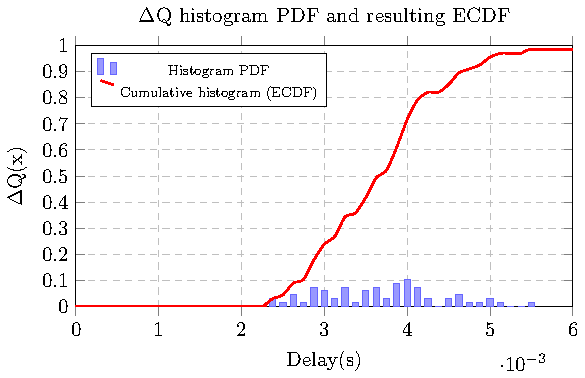
\includegraphics[scale=1]{tikz/pdf_dq.pdf} 
            \end{center}
            \caption{Blue bins: PDF of a sample $\Delta$Q. Red: Resulting CDF of $\Delta$Q PDF.}
        \end{figure}
 
    \subsection{dMax = $\Delta$t $\cdot$ N}
        The key concept of $\Delta$QSD is having a maximum delay after which we consider that the execution is timed out, consequently, it represents a failure. This is represented in the oscilloscope as $dMax$. Understanding this equation is key to correctly using the oscilloscope and exploring tradeoffs

Setting a maximum delay for a probe is not a job that can be done one-off and blindly, it is something that is done with an underlying knowledge of the system inner-workings and must be thoroughly fine-tuned during the execution of the system by observing the resulting distributions of the obtained $\Delta$Qs. 

Let us explain the following equation:
\begin{equation}
    dMax = \Delta t \cdot N  
    \label{eq:dMaxU}
\end{equation}

    \begin{itemize}
        \item $dMax$: The maximum delay, it represents the maximum delay that an outcome instance of a probe can have. The execution is considered "timed out" (failure) after $dMax$.
        \item $\Delta t$: The resolution of a $\Delta$Q. It is the bin width of a bin in a probe's $\Delta$Q.
        \item $N$: The precision of a $\Delta$Q. It is the number of bins in a probe's $\Delta$Q.
    \end{itemize}
    
    It can be informally described as a "two out of three" equation. If the user wants higher precision but the same $dMax$, the resolution must change, and so on for every parameter.
        \begin{figure}[H]
            \centering
            \begin{subfigure}{.5\textwidth}
                \centering
                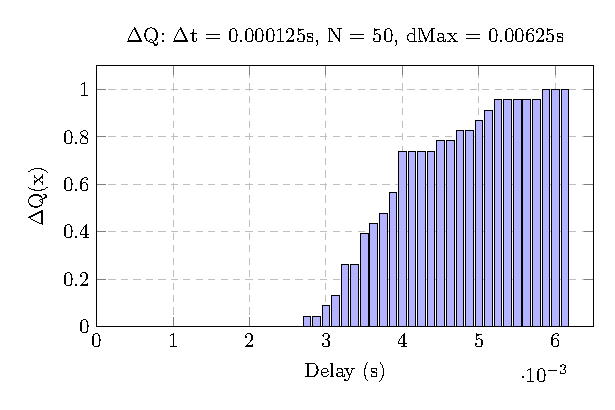
\includegraphics[width =0.98\textwidth]{tikz/hist_50.pdf}
                \label{fig:hist_50}
            \end{subfigure}%
            \begin{subfigure}{.5\textwidth}%
                \centering%
                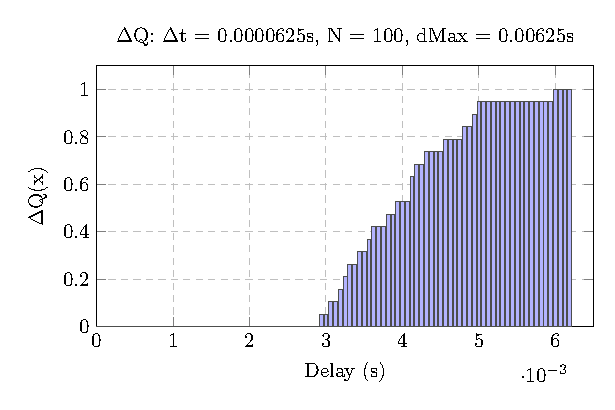
\includegraphics[width =0.98\textwidth]{tikz/hist_100.pdf}%
                \label{fig:hist_100}%
            \end{subfigure}%
            \label{fig:hist_dmax}%
            \caption{Left: Sample $\Delta$Q with higher resolution but lower precision. \\
            Right: Sample $\Delta$Q with lower resolution but higher precision. \\
            Both $\Delta$Qs have the same $dMax$, but the amount of precise information they provide is far different.}
        \end{figure}%

Some tradeoffs must though be acknowledged when setting these parameters, a higher number of bins corresponds to a higher number of calculations and space complexity, a lower $dMax$ may correspond to more failures. The user must set these parameters carefully during execution y observing the shown plots.

    \begin{figure}[H]
        \begin{center}
            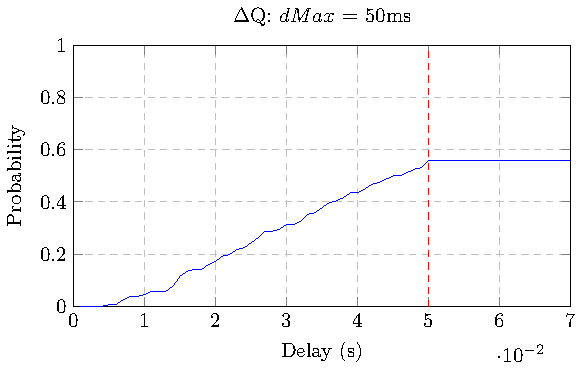
\includegraphics[scale = 1]{tikz/cdf_dmax.pdf}
        \end{center}
        \caption{$\Delta$Q: $dMax$ = 50ms, the $\Delta$Q will stay constant when delay $> dMax$.}
    \end{figure}

    \subsubsection{dMax limitation}
        $dMax$ can \textbf{not} be lower than 1 millisecond and will be rounded to the \textbf{nearest} integer in the adapter, this is a limitation of Erlang \texttt{send\_after} function which only accepts integers and milliseconds values. For example, if on the oscilloscope the $dMax$ is equal to $1.56 ms$, the adpater will fail spans after 2 ms.

    \subsection{QTA}
        A simplified QTA is defined for probes. We define 4 points for the step function at 25, 50, 75 percentiles and the maximum amount of failures accepted for an observable. An observed $\Delta$Q will calculate that based on the samples collected. 

\subsection{Confidence bounds}
    To observe the stationarity of a system we must observe the $\Delta$Qs of a probe over a polling window and calculate confidence bounds over those $\Delta$Qs. The bounds can be updated dynamically by inserting or removing a $\Delta$Q. They are removed when \#$\Delta$Qs(window) $>$ limit and added when calculating a new $\Delta$Q in a sampling window. \\
    This allows us to consider a small window of execution rather than observing the whole execution, this can help in observing stationarity of the system.
        \begin{figure}[H]
            \begin{center}
                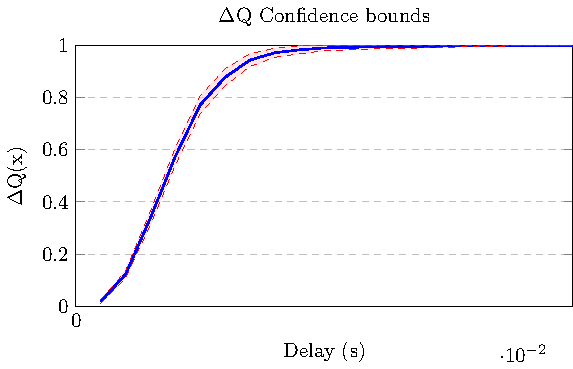
\includegraphics[scale=1]{tikz/ci.pdf} 
            \end{center}
            \caption{Upper and lower bounds (dashed, red) of the mean (blue) of multiple $\Delta$Qs. In a system that behaves linearly, the bounds will be close to the mean, once the overload is approaching, or a system is showing behaviour that diverges from a linear one, the bounds will be larger.}
        \end{figure}

  
